% Adjust these for the path of the theme and its graphics, relative to this file
%\usepackage{beamerthemeFalmouthGamesAcademy}
\usepackage{../../beamerthemeFalmouthGamesAcademy}
\usepackage{multimedia}
\graphicspath{ {../../} }

% Default language for code listings
\lstset{language=C++,
        morekeywords={each,in,nullptr}
}

% For strikethrough effect
\usepackage[normalem]{ulem}
\usepackage{wasysym}

\usepackage{pdfpages}

% http://www.texample.net/tikz/examples/state-machine/
\usetikzlibrary{arrows,automata}

\newcommand{\modulecode}{COMP260}\newcommand{\moduletitle}{Distributed Systems}\newcommand{\sessionnumber}{5}

\begin{document}
\title{\sessionnumber: Presence}
\subtitle{\modulecode: \moduletitle}

\frame{\titlepage} 

\begin{frame}
	\frametitle{Learning outcomes}
	\begin{itemize}
		\item Outcome 1
		\item Outcome 2
		\item Outcome 3
	\end{itemize}
\end{frame}

\begin{frame}
	``We see things not as they are, but as we are - that is, we see the world not as it is, but as moulded by the individual peculiarities of our mind'' \\~\\ - Philosopher, G.T.W Patrick. (1890) \\~\\
	\pause
	Reality is malleable. \\~\\ 
	\pause
	Our point of view is inseparable from our understanding of reality. 	
	
\end{frame}

\begin{frame}
	\begin{figure}
		\href{https://www.youtube.com/watch?v=gvozcv8pS3c}{ 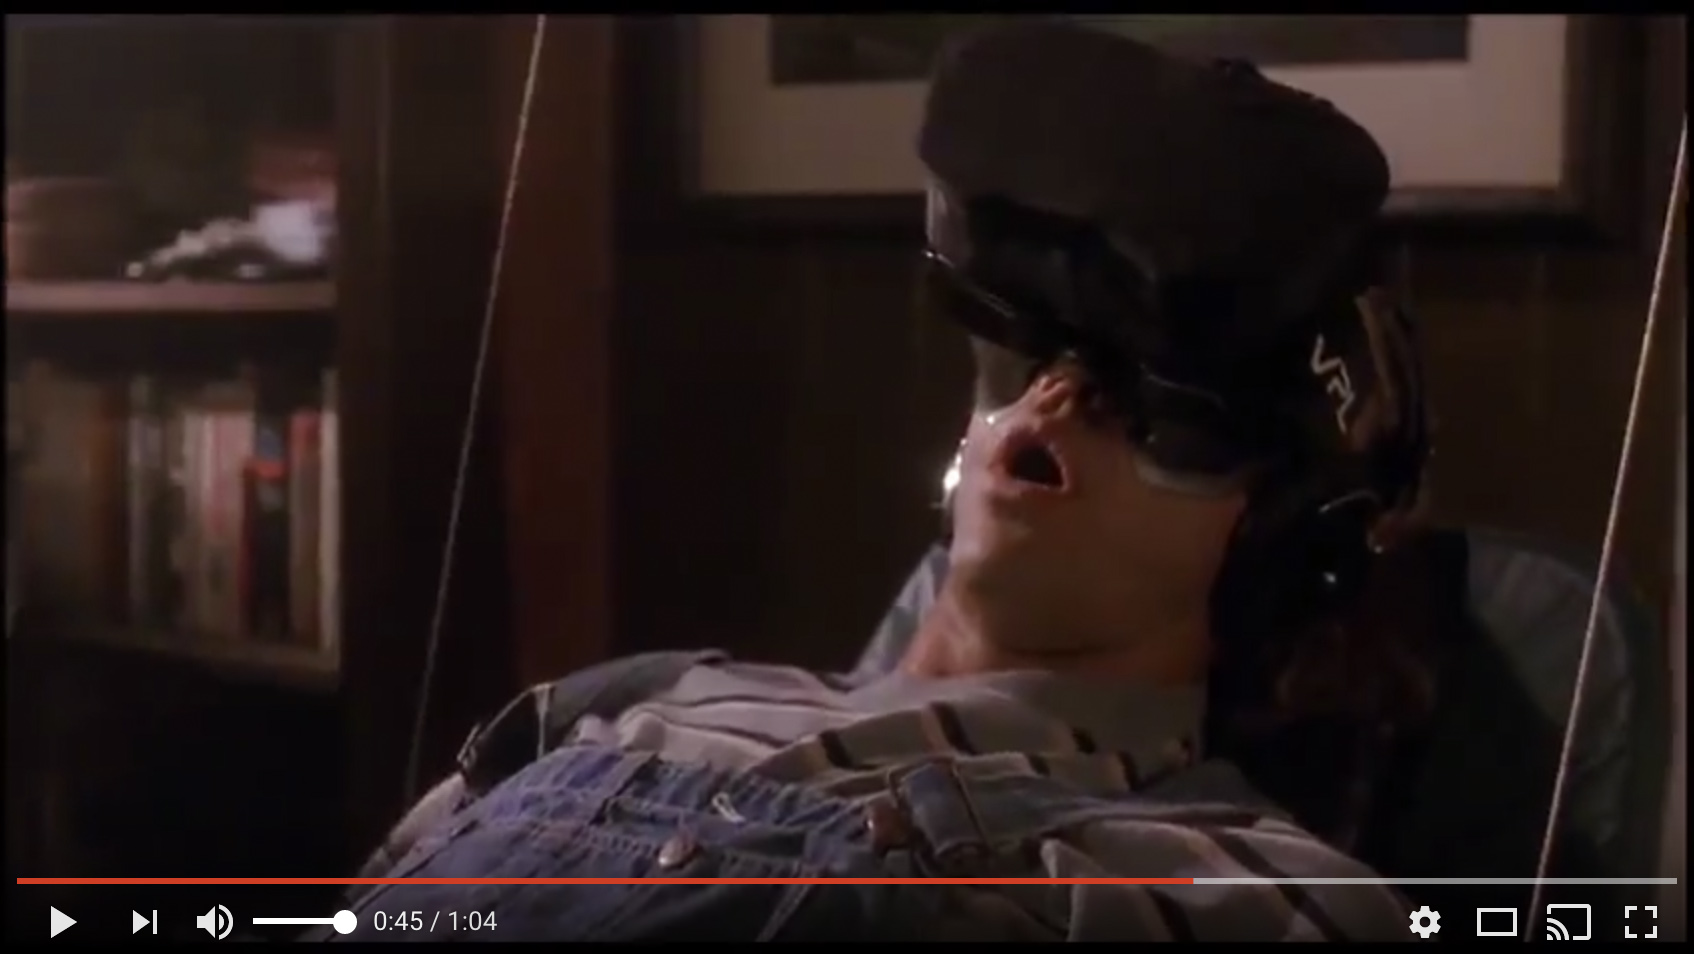
\includegraphics[scale=.3]{assets/mower}  }
		\caption{The Lawn Mower Man - 1992}
	\end{figure}
\end{frame}

\begin{frame}
	\frametitle{Duck Test}
	``a colloquial name for a method of testing if an experiencer has reached a state of presence, by monitoring their behaviour when threatened by a virtual object'' \\~\\
	- \href{http://www.vrglossary.org/glossary/duck-test/}{VRGlossary.org} \\~\\
	This could have an adverse effect if the experiencer realises that there is no actual risk - Presence is then broken.
		
\end{frame}


\begin{frame}
	\frametitle{Presence (again)}
	
	`Presence is the psychological state of subjective perception in which even though part or all of an individual's current experience is generated by and/or filtered through human-made technology, part or all of the individual's perception fails to accurately acknowledge the role of the technology in the experience.' \\~\\
	
	International Society for Presence Research, 2000
	\\~\\
	\href{http://ispr.info}{[ISPR Website]}	
	
\end{frame}


\begin{frame}
	\begin{figure}
		\href{https://www.youtube.com/watch?v=qD3w3cAhEYU}{ 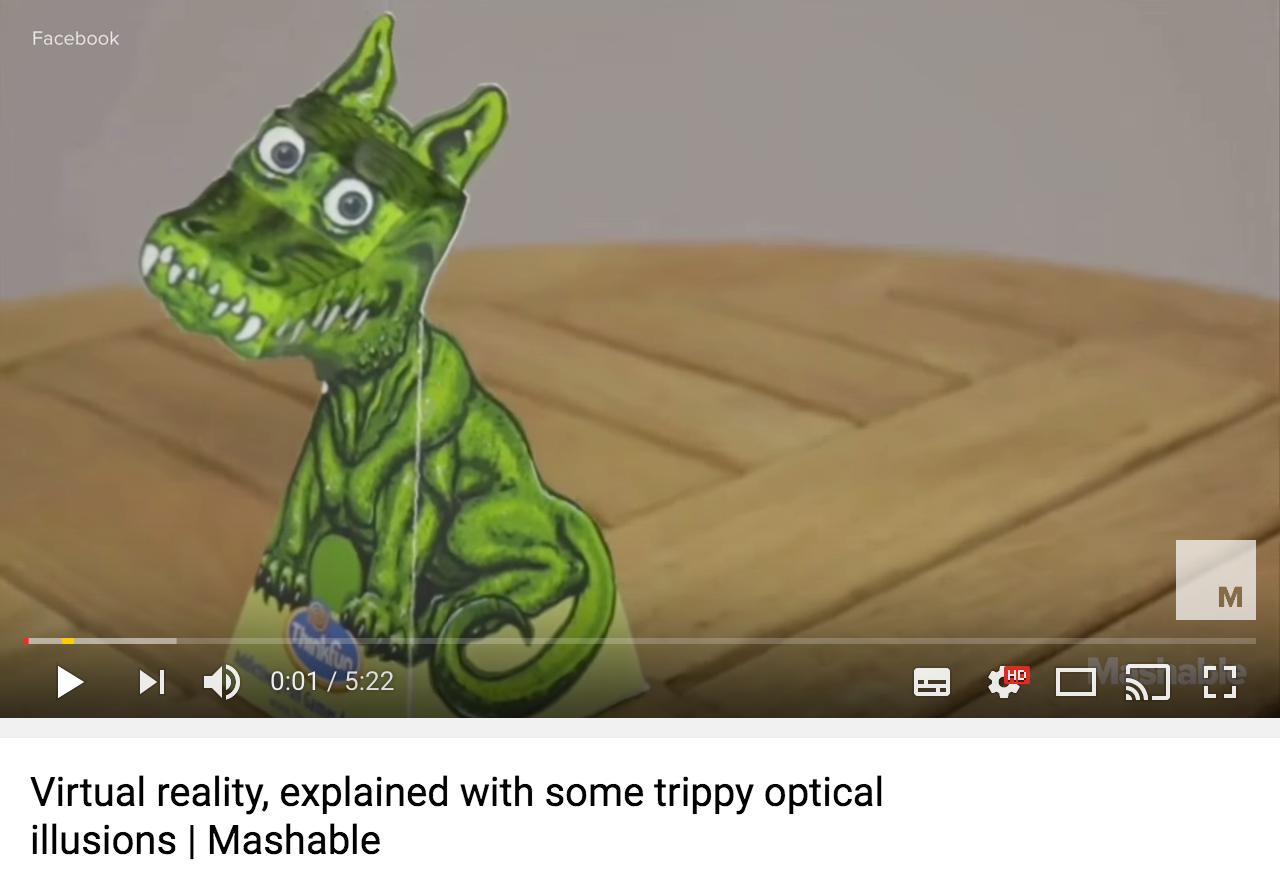
\includegraphics[scale=.4]{assets/optical}  }
		\caption{Michael Abrash, the chief scientist for Facebook's Oculus}
	\end{figure}
\end{frame}

\begin{frame}
	\frametitle{Activity}
	\textbf{Who can find the best optical illusion?} \\~\\
	
	Post results to Slack
	
\end{frame}

\begin{frame}
	\frametitle{Types of Illusion}
	\begin{itemize}
		\item Boundary Completion
		\item Blind Spot \href{http://snowbrains.com/wp-content/uploads/2013/07/eyeball.jpg}{ (link to eye)}
		\item Depth Illusions
		\item Afterimage
		\item Motion Illusions - Watch these in VR as they cause motion sickness. 
	\end{itemize}
\end{frame}

\begin{frame}
	\frametitle{Gestalt Psychological factors}
	Gestalt = Configuration (roughly)
\end{frame}

\begin{frame}
	\frametitle{Illusions}
	V/AR are illusion based experiences \\~\\ 
	
	There are four main components to this illusion:
	\begin{itemize}
		\item the stable spacial place,
		\item self-embodiment,
		\item physical interaction \&,
		\item social communication.
	\end{itemize}
\end{frame}


\begin{frame}
	\frametitle{Sensation vs. Perception}	
	\begin{figure}
		\href{https://youtu.be/Ebwtq1HZJ2A?t=1051}{ 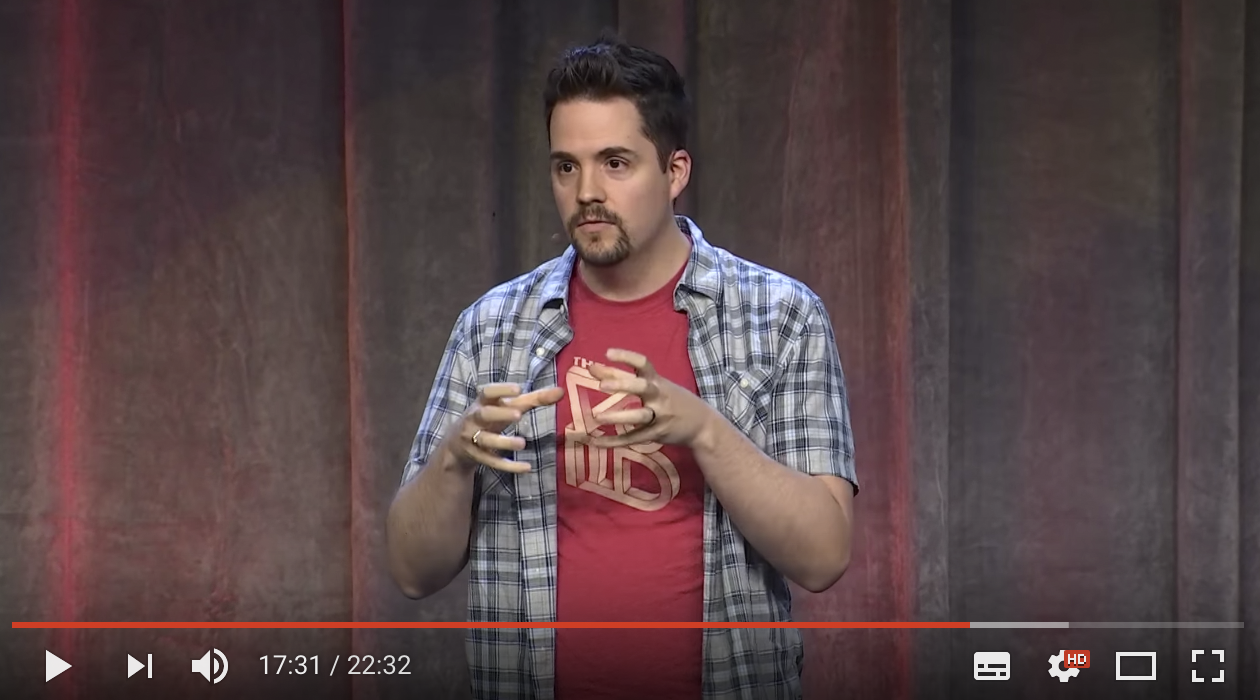
\includegraphics[scale=.4]{assets/sensation}  }
	\end{figure}
	\textbf{Sensation} - Lower level recognition of stimuli.
	\textbf{Perception} - Higher level processing that combines information from the senses, filters it, organises it then interprets it to create \textbf{subjective}, conscious experience. 
\end{frame}


\begin{frame}
	\frametitle{Objective \& Subjective Reality}
	
\end{frame}


\begin{frame}
	\frametitle{The Uncanny Valley}
	\begin{figure}
		 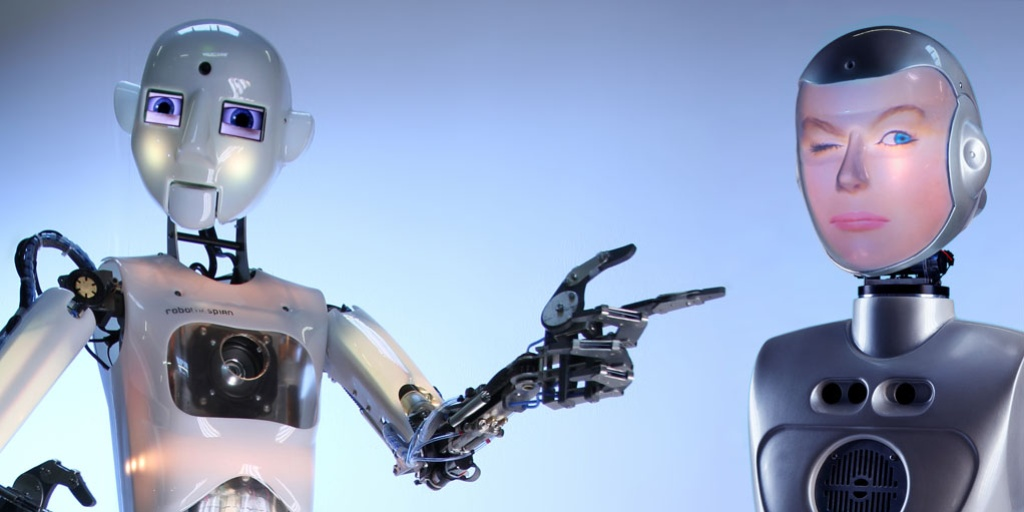
\includegraphics[scale=.3]{assets/bots}  
		 \caption{Engineered Arts - Penryn}
	\end{figure}
\end{frame}

\begin{frame}
	\begin{figure}
		 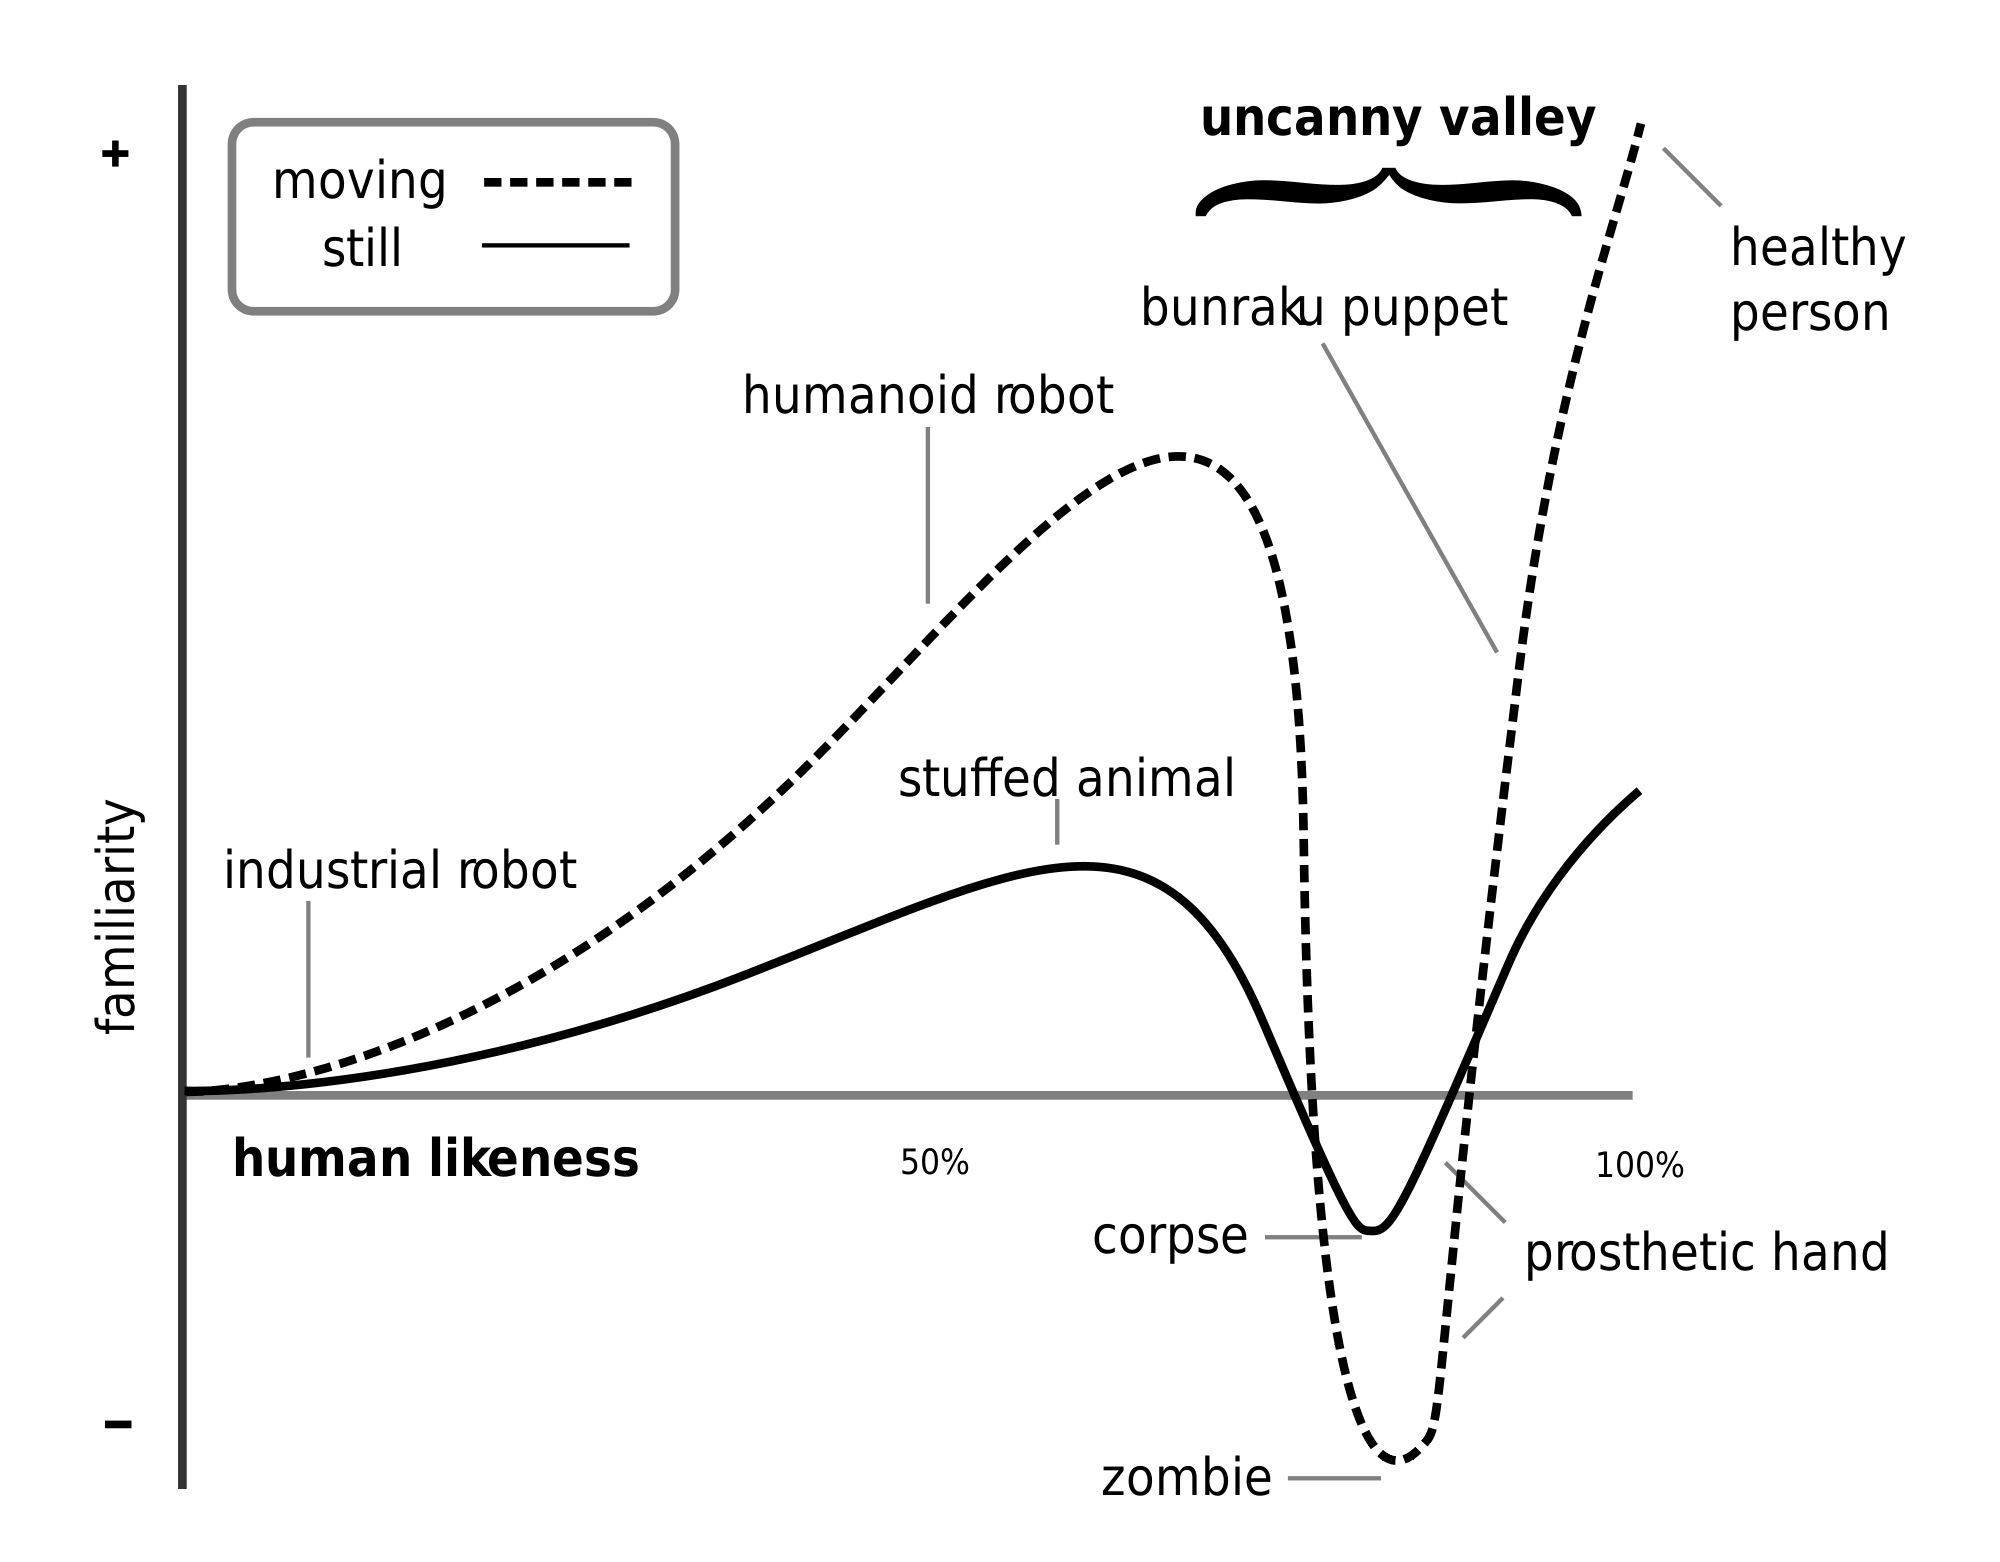
\includegraphics[scale=.13]{assets/uncanny}  
		  \caption{Masahiro Mori - }
	\end{figure}
\end{frame}

\begin{frame}
	\frametitle{Fidelity Continua}
	The notion of the uncanny valley applies to aspects of VR as well. These components have been defined as the Fidelity Continua. 
	
	\begin{itemize}
	 	\item	\textbf{Representation} fidelity - Hyper-realistic to abstract and non-objective worlds. 
		\item	\textbf{Interaction} Fidelity - Degree to which a interaction in VR corresponds with the same interaction in the real world.
		\item \textbf{Experiential} Fidelity - The degree to which the user experience matches the intentions of the VR creator. Procedural worlds have a very low experiential fidelity.
	 \end{itemize}
		
\end{frame}

\begin{frame}
	What do we want from V/AR? \\~\\
	Some aim to recreate reality to the highest fidelity. \\~\\
	Others seek to surpass it.
\end{frame}

\begin{frame}
	\frametitle{Sensory Substitution}
	Sensory substitution is the replacement one sensory cue that is not yet able to be simulated with one that is. 
	\begin{itemize}
		\item Ghosting - showing the user a second version of a virtual object. 
		\item Highlighting - Visual signifiers that convey a sense of interactivity with an object.
		\item Audio cues - Useful for identifying collisions with virtual objects.  
		\item Passive haptics - Real world reference frames meet virtual reference frames to help a user navigate a space. 
		\item Rumbles/sub packs - Again, used to portray a collision with virtual objects. 
	\end{itemize}
\end{frame}


\begin{frame}
	\frametitle{Misdirection}
	``That which directs a spectator away from the method and towards the effect'' \\~\\
	Curtis Hickman - Magician \& founder of THE VOID. \\~\\
	TRUTH/REALITY \textgreater  GUIDED PERCEPTION \textgreater  LIE/FANTASY \\~\\
	\href{https://www.youtube.com/watch?v=Ebwtq1HZJ2A}{LINK}
\end{frame}
	
\begin{frame}
	\frametitle{Redirected Walking}
	\begin{figure}
		\href{https://www.youtube.com/watch?v=qD3w3cAhEYU}{ 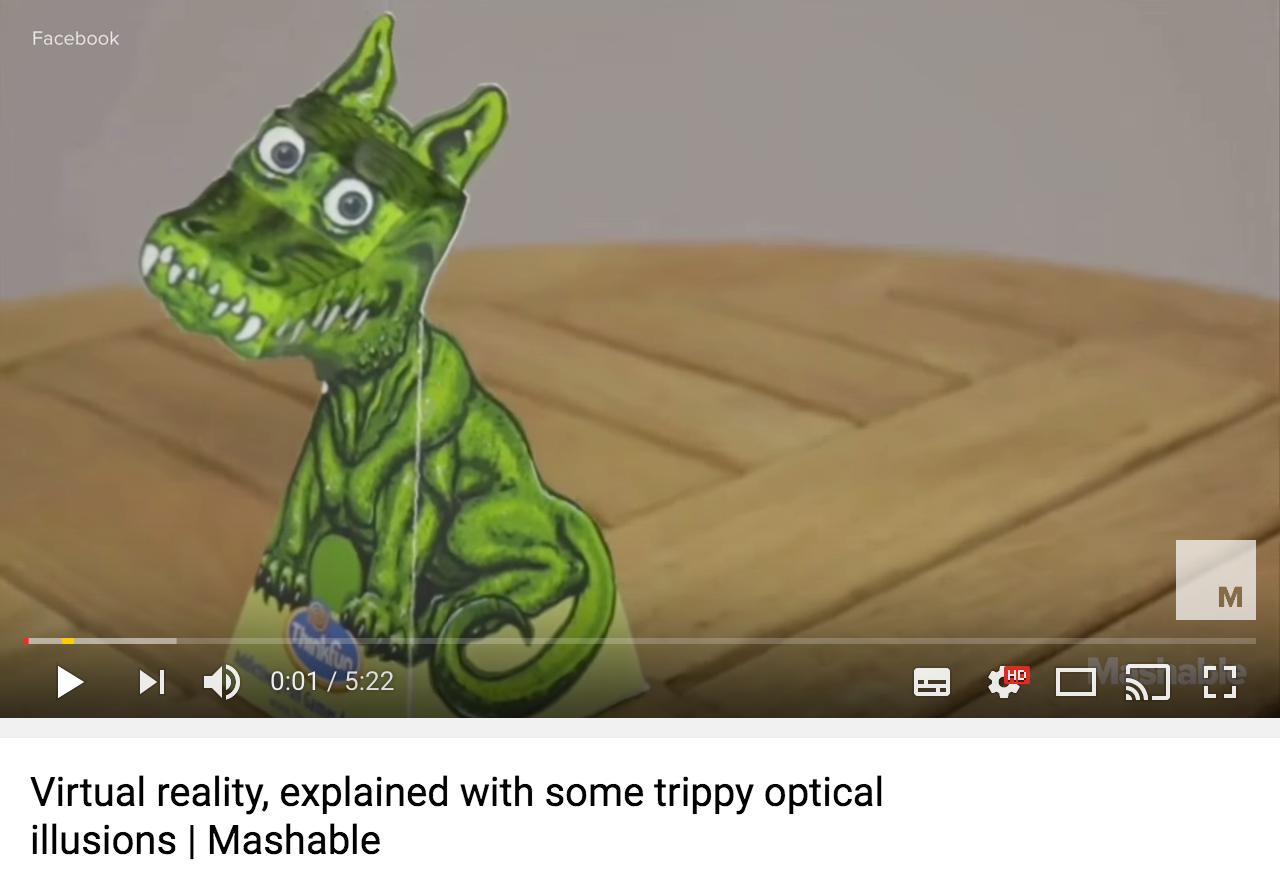
\includegraphics[scale=.4]{assets/optical}  }
		\caption{Michael Abrash, the chief scientist for Facebook's Oculus}
	\end{figure}
	``HUMANS, QUITE SIMPLY, suck at walking in straight lines'' Wired Magazine
	
\end{frame}


\end{document}
